%------------------------------------------------------------------------%
% Example figure for the thesis template.                                %
%                                                                        %
%      Author: Gregory Alexander Feiden                                  %
%   Institute: Dartmouth College                                         %
%        Date: 2014 May 17                                               %
%                                                                        %
%     License: Beerware (revision 42)                                    %
%              ----------------------                                    %
%              Gregory Feiden wrote this file. As long as you retain     %
%              this notice you can do whatever you want with this code.  %
%              If we meet some day and you think this code is worth it,  %
%              you can buy me a beer in return.                          %
%                                                                        %
%------------------------------------------------------------------------%

\begin{figure}[t]
    \begin{center}
        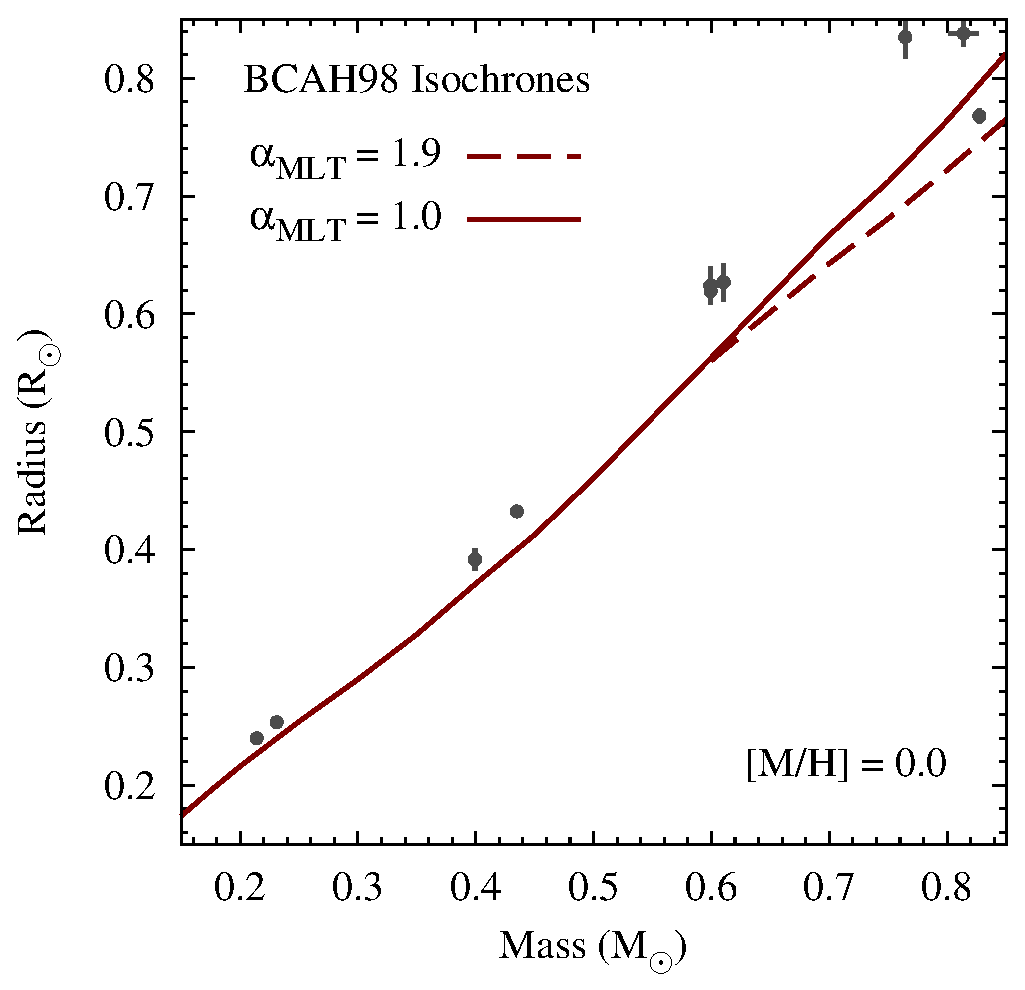
\includegraphics[scale=0.42]{./ch1/fig/bcah_1_gyr_MR.eps}
        \hspace{\fill}
        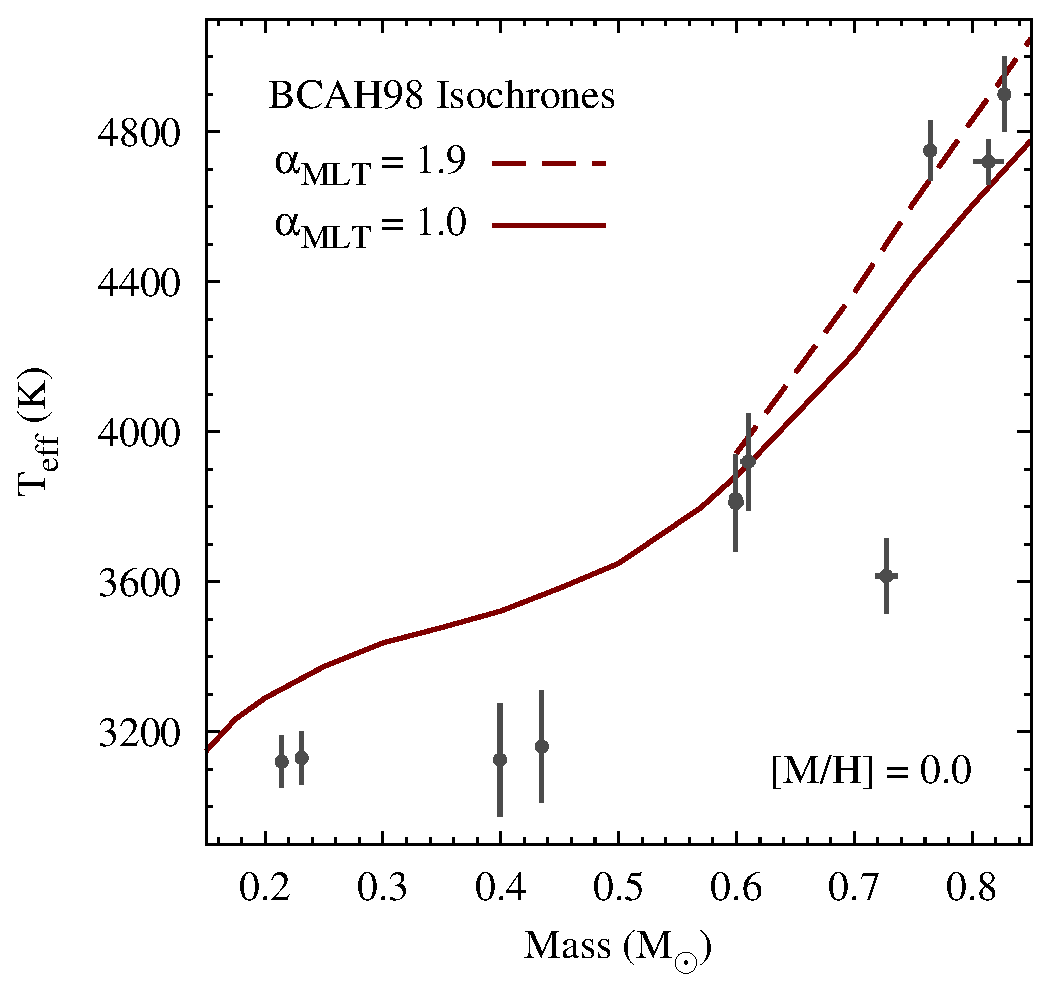
\includegraphics[scale=0.42]{./ch1/fig/bcah_1_gyr_MT.eps}
        \caption[Example of a simple figure.]
        {An example of a two panel figure. Naturally, there can 
         be as few or as many panels as you'd like. All figures 
         will be numbered Chapter.Section and will be refered to
         as such using the ``label--reference'' system. Additionally,
         there is no need for figures to be on separate pages in
         a Dartmouth thesis, it's up to the author.}
        \label{fig:example1}
    \end{center}
\end{figure}
